\chapter{Proposition of new model}

\label{chap:research}

The aim of this thesis was to create a new semi-supervised model. The concept which we decided to include in this new model is self-organization. Self-organizing models do not need labels to learn data topology, so it is suitable for all training data of semi-supervised models - labeled and also unlabeled. This chapter contains steps toward the proposition of the model, such as the selection of a self-organizing model, the designing of a new semi-supervised model and the definition of its crucial parts, which will be investigated in the following chapters.

The unsupervised part of the loss function in semi-supervised learning is mostly based on prediction consistency. In case of the Mean Teacher model, this consistency is between predictions of the teacher and student model. Other models, for example, the Siamese neural network, hold consistency between predictions of one model on a sample augmented in two different ways.

\section{Unsupervised model selection}
In our research, we decided to use a Self-organizing map (SOM)\cite{kohonen1990} for the evaluation of the consistency of data points from the same class. A self-organizing map was described in section \ref{sec:som}. SOM was used as an unsupervised component of the loss function. Unlike other unsupervised techniques, SOM can provide a nonlinear transformation of the input into the low-dimensional grid. Another advantage of SOM is that it is neural network based, so its complexity is scalable. We expected that clustering using SOM could be useful to determine the similarity of training examples.


\section{Related work}
Since we came up with this concept of using a Self-organizing map as auxiliary information for a semi-supervised model, we searched for similar concepts in the literature and found few models, that used SOM in combination with another model, such as mnSOM \cite{Tokunaga}, Tamazirt`s model \cite{Tamazirt} or DESOM model \cite{desom2019}.

Tokunaga and Furukawa \cite{Tokunaga} proposed a model that connects SOM and supervised model, for example, MLP in a generalized framework called the modular network SOM (mnSOM). The mnSOM consists of trainable MLPs that are used instead of vectors representing the data prototypes, therefore moving the functionality of the SOM model towards multi-objective learning that captures the organization in a function space rather than in vector space. The training of the MLP is separated from the training of the SOM. 

Another model that utilizes both an MLP and SOM was proposed in a very specific application of intelligent indoor 3D positioning by Tamazirt and colleagues \cite{Tamazirt}. In their model, the adapted SOM is paired with several MLP networks. It serves for clustering and does not directly interfere with the learning in the MLPs. 

The one most worth explaining is the model Deep Embedded Self-Organizing Map \cite{desom2019}, which includes the SOM layer in auto encoder model and defines loss function based on SOM.


\subsection{DESOM model}

Forest et al. \cite{desom2019} introduced a model called  Deep Embedded Self-Organizing Map (DESOM). The authors combined two unsupervised models - autoencoder and SOM. The combined model was trained in an unsupervised setup and achieved good results in the clustering task. Clusters were taken from the SOM part of the model. It was the first ever usage of SOM in a deterministic autoencoder model. The proposed model architecture can be seen in Figure \ref{fig:desom}. 


\begin{figure}[h!]
        \centering
        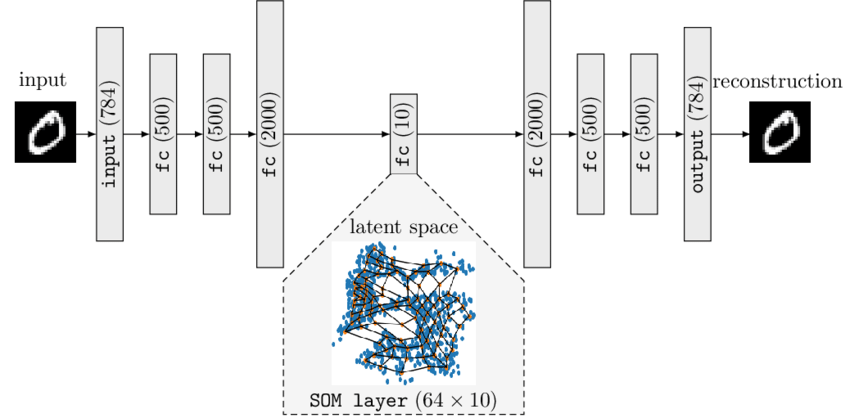
\includegraphics[width=1\textwidth]{figs/DESOM-architecture-with-an-8-8-map.png}
        \caption{DESOM model architecture \cite{desom2019}}
        \label{fig:desom}
\end{figure}

DESOM model uses combined loss in encoder network training - the weighted sum of reconstruction loss $\mathcal{L}_r$, which is conventionally used in autoencoder, and SOM loss $\mathcal{L}_{som}$.
SOM loss is defined as $$\mathcal{L}_{som} = \sum_i \sum_{k=1}^K \mathcal{K}^T (\delta (\mathcal{X}(f_{W_e}(x_i)), k)) {||f_{W_e}(x_i) - m_k||}^2,$$ where neurons in SOM are numbered from $1$ to $\mathcal{K}$ and weights of $k$-th neuron are denoted $m_k$. $\mathcal{K}^T$ is neighbour function dependant on time $T$ which computes neighbourhood relationship based on position difference $\delta$ between $k$-th neuron and position of winner neuron $\mathcal{X}(f_{W_e}(x_i))$ for $i$-th input.
The decoder part is trained only using $\mathcal{L}_r$. SOM is trained using $\mathcal{L}_{som}$. The authors used no pre-training.

In their experiments, they focused on unsupervised clustering accuracy (using the SOM part of the model), in which DESOM has the best results in all three datasets (MNIST \cite{deng2012mnist}, Fashion-MNIST \cite{xiao2017fashionmnist}, REUTERS-10k a text dataset built from the RCV1-v2 corpus \cite{rcvi}). They also examined Purity and NMI matrices, in which the model compared with other clustering models achieved the best in the majority of the cases best results.

This article brought us $3$ findings important for our research. First, that it is possible to use some kind of extracted information (latent space representation of autoencoder) as input for SOM, and the results are really good. Second, it is possible to train SOM on changing inputs and it still clusters data properly. And third, the usage of another model can improve the model in its task. These results supported our intuition, that self-organization of data can also improve the performance of semi-supervised models.


\section{Our approach}
\label{our-approach}
We extended the semi-supervised model Mean Teacher described in section \ref{mtm-chapter} and introduced the MT-SOM model. MT-SOM model is based on three main new concepts, which are feature vector representation, pre-trained Self-organizing map and mean teacher model with SOM-based consistency loss.

Our semi-supervised MT-SOM model is composed of two neural networks (student and teacher) with the same layer architecture, but separate trainable weights. For each training sample, the forward pass of both networks is done and produced feature vectors are used for computation of consistency cost \color{red} označenie \color{black}, which is SOM SOM-based loss function. The output of the student network is used for supervised cost \color{red} označenie \color{black} computation, which is the Mean squared error of prediction and label, but only in the case of labeled input sample. Then, both losses are combined together and backward pass with weight update based on this final value of loss provided in the student's network. The teacher network is updated in the same way as in the Mean teacher model, it is an Exponential moving average of student. The proposition of our model is graphically shown in Figure \ref{fig:our-model}. 

\begin{figure}[h!]
    \centering
    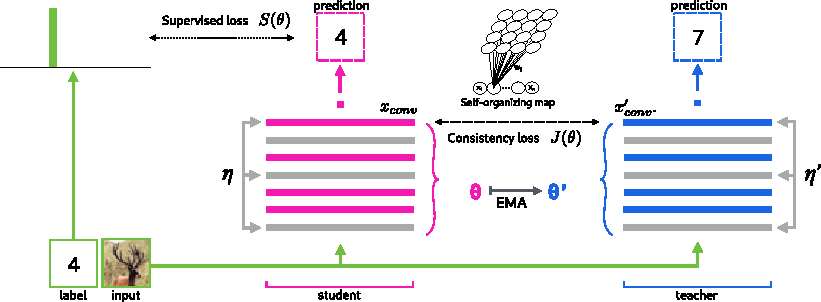
\includegraphics[width = 1\textwidth]{figs/mean_teacher_som-1.pdf}
    \caption{Description of MT-SOM model}
    \label{fig:our-model}
\end{figure}


\color{red} zjednotit oznacenia v rovnici a obrazku !!!!! \color{black}


\subsection{Feature vector representation}
The idea of using feature vectors - representation of input after the last convolutional layer of model - instead of predictions for unsupervised cost is from Binary mean teacher research \cite{tuna-bmt} and it is also supported by our research in previous chapter \ref{chap:bmt-exp} and DESOM research. We decided to use it since it worked well for the BMT model and we suppose it can contain more information than prediction because it has a higher dimension than the output vector and still contains only extracted features that are important for classification.

To strengthen our intuition, that SOM is able to cluster MT feature vectors properly, we took implementation of Mean Teacher from authors GitHub repository \cite{curiousai} and produced feature vectors for setup that declared state-of-the-art results. The input dataset for MT was the standard dataset CIFAR-10 previously described in section \ref{dataset-cifar10}, which contains color images from $10$ classes. Then we used feature vectors as inputs for SOM. SOM was trained in unsupervised setup for $30$ epochs and the two-dimensional map was visualized in figure \ref{fig:som-cluster-mt}. We can see that neurons are quite well organized. Further investigation of the difference between original CIFAR-10 versus feature vectors from MT as the input is in chapter \ref{chap:som-fv-cifar}.

\begin{figure}[h!]
    \centering
    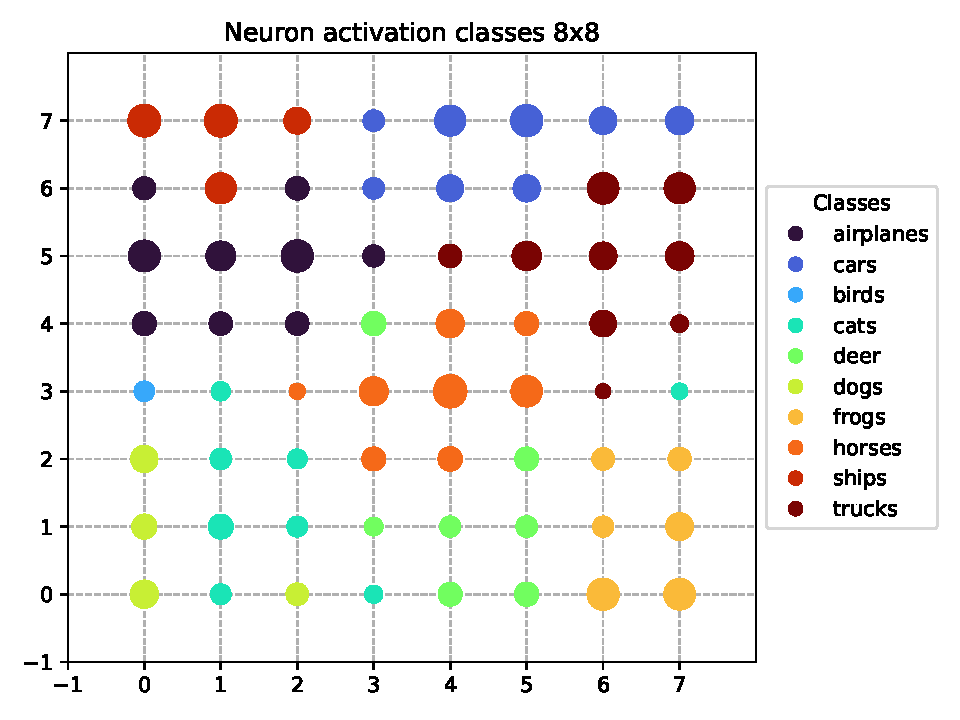
\includegraphics[width=0.9\textwidth]{figs/som-clusters-mt.pdf}
    \caption[SOM clusters from MT feature vectors]{In the legend, we can see $10$ classes of dataset CIFAR-10. Dots in the graph show properties of neurons in $8\times8$ grid. Color means class which neuron represents and size means percentage of input vectors from this class from all inputs represented by this neuron as their winner neuron. We can see, that space is organized into clusters and all inanimate object clusters are in the upper part. Animate object clusters are in the lower part. Also, we can see that a cluster of airplanes is right next to neuron that represents birds. We can see one bigger outlier from the deer class in the middle, but we can explain it by looking at what is in between this outlier and the deer cluster. It is a horse cluster, so since these creatures are quite similar, it can be an explanation for this outlier.}
    \label{fig:som-cluster-mt}
\end{figure}


\subsection{Pre-trained Self-organizing map}

From the DESOM paper, we knew that there exists a setup, where it is possible to co-train supportive SOM on changing inputs from another neural network. However, we believe, that this part of the model could cause the biggest complications in model development. We decided to use a pre-trained Self-organizing map instead. 

The inputs of SOM are crucial, as we decided to use feature vectors as input of SOM, we needed to achieve them at the beginning of the training. Hence, we pre-trained the student network of the Mean teacher model in a supervised way with labeled part of the training dataset. Then we did a forward pass for each training sample, no matter if it was labeled or unlabeled, and saved feature vectors. This set of feature vectors was our training dataset for SOM training. We pre-trained the SOM model on it. 

In the chapter \ref{chap:mlp-som}, we tested this concept of pre-trained SOM model usage in a more simple setup, where we used table data. Table data does not need to be transformed into feature vectors by convolutions neural network, since they are not images. So in the experiment, we used only vanilla input data.


\subsection{SOM-based consistency loss}
Another crucial component of the model was new consistency loss, which should have taken into account the distances of winner neurons of two data points on the SOM map. Since SOM clusters data, we believed, that if data are unlabeled, this topological information can help in their classification. As described in the DESOM section, there was a proposition for SOM-based loss function. We were inspired by this research in some way, but introduced and tested custom SOM losses in chapter \ref{chap:mlp-som} for the supervised model and \ref{chap:mt-exp} for the unsupervised model.


\section{Sub-experiments}
Since we introduced a new model with many hyperparameters, experimental investigation of all of them with different combinations of values would have extremely high computational demand and could end with unsure results. Our solution was to investigate the main components of the MT-SOM model separately and in more simple setups. Based on developed knowledge, we planned to choose good parts of setups and combine them into the final model.

The following two chapters are dedicated to SOM-based consistency loss development and feature vector usage as SOM inputs. In chapter \ref{chap:mlp-som}, we look at the supervised model using auxiliary SOM-based loss and its accuracy compared to the baseline model without this auxiliary information.
In chapter \ref{chap:som-fv-cifar}, we compare SOM qualitative and quantitative metrics in the case when image dataset is used, versus when feature vectors of images are used.